\documentclass[a4paper,12pt,bibtotoc, parskip=full]{article}
\usepackage[top=2.2cm, bottom=2.5cm, left=2cm, right=2cm]{geometry}
\usepackage[pdftex]{graphicx}
%\usepackage[ngerman]{babel}
\usepackage[german,ngerman]{babel}
\usepackage[utf8]{inputenc}
%\usepackage{fontspec}
%\usepackage{xunicode}
%\usepackage{xltxtra}
\usepackage{booktabs}
\usepackage{tabularx}
\usepackage{amsmath,amssymb}
\usepackage{amsfonts}
\usepackage{hyperref}
\usepackage{floatflt}
\usepackage{flafter}
\usepackage{color}
\usepackage{rotating}
\usepackage[centerlast]{caption}
\usepackage[toc,page,title,header]{appendix} 
\usepackage{setspace}
\onehalfspacing

\usepackage{textcomp}

\renewcommand{\appendixtocname}{Appendizes}
\renewcommand{\appendixpagename}{Appendizes}


\newtheorem{defi}{Definition}
\newtheorem{satz}{Satz}

\setcounter{tocdepth}{2}
\begin{document}
\begin{titlepage}
\title{Pflichtenheft - iPhone App Texas Hold'em}
\author{iOS-Fortgeschrittenenpraktikum - Gruppe 2}
\maketitle
\vspace{10cm}
\centering{Auftraggeber:\\Lehrstuhl für Informatik V\\ Prof. Dr. Reinhard Männer\\ Uni Heidelberg}
\thispagestyle{empty}
\end{titlepage}
\newpage
\thispagestyle{empty}
\tableofcontents
\newpage
\setcounter{page}{1}

\section{Zielbestimmung}
Die Poker iPhone App ist ein Spiel für das iPhone. Der Benutzer kann damit das Pokerspiel 'Texas Hold'em' gegen andere Benutzer und/oder gegen Computergegner spielen.

\subsection{Musskriterien}
\begin{itemize}
\item Startbildschirm
    \begin{itemize}
    \item Nach dem Start der App wird ein Startbildschirm angezeigt, der den Namen der App anzeigt
    \end{itemize}
\item Der Benutzer
    \begin{itemize}
    \item Der Benutzer kann zunächst zwischen folgenenden Menüs wählen: Einstellungen, Singleplayer und Multiplayer
    \item Einstellungen: Der Benutzer kann seinen Spielernamen eingeben/ändern und ein Avatar oder Bild festlegen
    \item Singleplayer: Der Benutzer kann die Anzahl der Computergegner (1--4) festlegen sowie die verfügbare Summe Geld und den Einsatz pro Runde (Blind)
    \item Multiplayer: Der Benutzer kann einem Multiplayerspiel beitreten oder ein Multiplayerspiel neu erstellen
    \item Wenn der Benutzer ein Multiplayerspiel selber erstellt, kann er die Anzahl der Mitspieler (1--4) festlegen sowie die verfügbare Summe Geld und den Einsatz pro Runde (Blind)
    \end{itemize}
\item Das Spiel
    \begin{itemize}
    \item Ein Spieler wird zufällig als Dealer ausgewählt. Der Spieler links von ihm wird aufgefordert den ersten Einsatz (small blind) zu machen, der nächste Spieler wird  aufgefordert, den normalen Einsatz (big blind) zu machen
    \item Der Spieler erhält zwei Karten
    \item Der Spieler kann an der ersten Wettrunde teilnehmen, in dem er aufgefordert wird zwischen den drei Optionen call, raise oder fold zu wählen
        \begin{itemize}
        \item call: Der Spieler setzt einen Betrag in Höhe des vorangegangenen Einsatzes
        \item raise: Der Spieler erhält die Möglichkeit, einen Betrag einzugeben, der über dem vorangegangenen Einsatz liegt
        \item fold: Der Spieler gibt diese Wettrunde auf und kann nur die offen gelegten Karten bis zum Ende der Runde sehen
        \end{itemize}
    \item Falls einer der Spieler 'raise' gewählt hat, erhalten alle anderen Spieler die Möglichkeit, die Differenz zu dem höchsten Einsatz auszugleichen oder diese Wettrunde aufzugeben
    \item Nachdem alle Spieler aufgefordert wurden, Ihre Auswahl zu treffen, endet die erste Wettrunde
    \item Nach dem Ende der ersten Wettrunde werden drei Karten offen angezeigt
    \item Die zweite Wettrunde beginnt wiederum mit dem Spieler links des Dealers
    \item Der Spieler erhält die Möglichkeit, zwischen drei Optionen zu wählen: check, bet und fold
        \begin{itemize}
        \item check: Der Spieler wartet auf die nächste Runde
        \item bet: Der Spieler erhält die Möglichkeit, einen Betrag einzugeben. Für alle anderen Spieler steht diese Option von nun an nicht mehr zur Verfügung
        \item fold: Der Spieler gibt diese Wettrunde auf und kann nur die offen gelegten Karten bis zum Ende der Runde sehen
        \end{itemize}
    \item  Nachdem alle Spieler aufgefordert wurden, Ihre Auswahl zu treffen, endet die zweite Wettrunde
    \item Nach dem Ende der zweiten Wettrunde wird eine vierte Karte offen ausgelegt
    \item Die dritte Wettrunde verläuft analog zur zweiten Wettrunde
    \item Nach dem Ende der dritten Wettrunde wird eine fünfte Karte offen ausgelegt
    \item Die vierte Wettrunde verläuft analog zur zweiten und dritten Wettrunde
    \item Nach dem Ende der vierten Wettrunde wird die beste fünf-Karten-Kombination jedes im Spiel verbliebenen Spielers ermittelt
    \item Der Spieler mit der höchsten Kombination wird bekanntgegeben und der gesamte Spieleinsatz aller Mitspieler aus allen Wettrunden wird seinem Konto gutgeschrieben
    \item Der Spieler links des Dealers wird der neue Dealer und eine neue Runde beginnt
    \item Hat ein Spieler kein Spielgeld mehr zur Verfügung wird ihm ein Bildschirm mit seiner Positionierung angezeigt
    \item Spezialfall 'All-in': Übersteigt der Einsatz der aktuellen Wettrunde das Restvermögen des Spielers, bekommt er die Möglichkeit 'All-in' zu wählen, wodurch er die laufende Runde beenden kann  
    \end{itemize}
\end{itemize}

\subsection{Wunschkriterien}
\begin{itemize}
\item Der Spieler kann seine bisherigen Platzierungen sehen und wieviel Geld er bisher insgesamt gewonnen/verloren hat
\item Eine Hilfsbildschirm, der die Kartenkombinationen nach Ihrer Wertigkeit aufzeigt
\item Der Spieler hat die Möglichkeit, Nachrichten an andere Spieler zu schicken
\item Computerspieler können gegen andere Computerspieler antreten
\item Der Spieler, der ein Multiplayerspiel eröffnet hat, hat die Möglichkeit, Mitspieler aus dem Spiel auszuschliessen und neue Mitspieler in das laufende Spiel einzuladen. 
\end{itemize}
\subsection{Abgrenzungskriterien}
\begin{itemize}
\item Es sollen keine Spielstände gespeichert werden.
\item Es werden keine 3D-Animationen verwendet.
\end{itemize}
\newpage


\section{Produkteinsatz}
\subsection{Anwendungsbereiche}
Es handelt sich um das Spiel Texas Hold'em, welches über iPhone von Einzelpersonen mit anderen Spielern über das Netzwerk  gespielt werden soll.

\subsection{Zielgruppen}
Leute, die Pokern möchten, aber keine Karten dabei haben oder die trotz örtlicher Entfernung miteinander spielen möchten\\
Die Spielregeln werden vorausgesetzt\\
Der Benutzer sollte deutsch verstehen
\newpage

\section{Produktumgebung}
\subsection{Hardware}
iPhone 4 und höher
\newpage

\section{Produktfunktionen}
\subsection{Benutzerfunktionen}

\textbf{/F0010/} Der Benutzer hat zu Beginn die Möglichkeit sich zwischen den Menüs Einstellungen, Singleplayer- und Multiplayerspiel zu entscheiden.\\
\textbf{/F0020/} Der Benutzer kann in den Einstellungen sein Bild und seinen Spielernamen verändern.\\
\textbf{/F0030/} Der Benutzer kann im Menü Singleplayerspiel die Anzahl der Spieler, die Anzahl der Computergegner und die Summe des verfügbaren Geldes pro Spiel für jeden Spieler festlegen.\\
\textbf{/F0040/} Dem Benutzer werden im Menü Multiplayerspiel Spiele angezeigt, denen er gegebenenfalls beitreten kann. Darüberhinaus hat der Benutzer die Option, ein neues Multiplayerspiel zu erstellen.\\
\textbf{/F0050/} Tritt der Benutzer einem Spiel bei, wartet er bis das Spiel beginnt.\\
\textbf{/F0060/} Startet der Benutzer ein neues Spiel, muss er die Anzahl der Mitspieler sowie die Summe des verfügbaren Geldes für alle Spieler festlegen.\\
\textbf{/F0070/} Hat ein Benutzer ein Spiel erstellt und wartet auf Spieler, kann er ein Spiel vorzeitig beginnen und die fehlenden Plätze mit Computergegnern auffüllen.\\

\subsection{Spielfunktionen}
\textbf{/F0110/} Zu Beginn des Spiels wird der Dealer zufällig ermittelt und allen Mitspielern mitgeteilt.\\
\textbf{/F0120/} Der Spieler links des Dealers wird aufgefordert den small blind zu setzen.\\
\textbf{/F0130/} Der nächste Spieler wird aufgefordert den big blind zu setzen.\\
\textbf{/F0140/} Wurde der big blind gesetzt, erhalten alle Spieler zwei Karten.\\
\textbf{/F0150/} Der Spieler erhält die Möglichkeit, zwischen den Optionen call, raise und fold zu wählen.\\
\textbf{/F0160/} Wählt ein Spieler call, wird ein Betrag in Höhe des aktuellen Höchstgebots vom Konto des Spielers abgezogen.\\
\textbf{/F0170/} Wählt ein Spieler raise, kann er einen Betrag angeben, der über dem aktuellen Höchstgebot liegt aber das verbliebene Menge Geldes des Spielers nicht überschreitet. Diese Funktion steht den nachfolgenden Spielern nicht mehr zur Verfügung.\\
\textbf{/F0180/} Wählt ein Spieler fold, scheidet er aus dieser Runde aus.\\
\textbf{/F0190/} Nachdem alle Spieler ihre Wahl getroffen haben (/F0150/), werden drei Karten für alle Spieler sichtbar angezeigt.\\
\textbf{/F0200/} Der Spieler erhält die Möglichkeit, zwischen den Optionen check, bet und fold zu wählen.\\
\textbf{/F0210/} Wählt der Spieler check aus, ist der nächste Spieler an der Reihe.\\
\textbf{/F0220/} Wählt der Spieler bet aus, kann er einen Betrag angeben, der über dem aktuellen Höchstgebot liegt aber das verbliebene Menge Geldes des Spielers nicht überschreitet. Diese Funktion steht den nachfolgenden Spielern nicht mehr zur Verfügung.\\
\textbf{/F0230/} == /F0180/\\
\textbf{/F0240/} Nachdem alle Spieler ihre Wahl getroffen haben (/F0200/), wird eine weitere Karte für alle Spieler sichtbar angezeigt.\\
\textbf{/F0250/} Die höchste Kombination aus den offen sichtbaren Karten und den beiden Karten des Spielers wird ermittelt und mit denen der anderen Spieler verglichen.\\
\textbf{/F0260/} Der Spieler mit der höchsten Kombination gewinnt die Runde und der gesamte Einsatz aller Spieler wird dem Konto des Gewinners gutgeschrieben.\\
\textbf{/F0270/} Der Spieler links des Dealers wird der neue Dealer für die nächste Runde.\\
\textbf{/F0280/} Wenn das Konto des Spielers 0 erreicht, scheidet er aus dem Spiel aus und ihm wird ein Schlussbildschirm mit seiner Positionierung angezeigt.\\
\textbf{/F0290/} Befindet sich der Spieler in einer der Wettrunden (/F0150/ bzw. /F0200/) und das aktuelle Gebot übersteigt die verbliebene Menge Geldes des Spielers, bekommt er die Optionen All-in und fold angezeigt. Alle anderen Optionen stehen für den Spieler dann nicht mehr zur Verfügung.\\
\textbf{/F0300/} Wurde die Option All-in von einem Spieler gewählt, nimmt er an den verbliebenen Wettrunden (/F0200/) nicht mehr teil. Er erhält allerdings weiterhin Karten (/F0240/) und spielt um den Gewinn der Runde mit (/F0260/).
\newpage

\section{Produktdaten}
\textbf{/D10/} Profildaten
\begin{itemize}
\item Spielername
\item Spielerbild
\end{itemize}
\textbf{/D20/} Spieldaten
\begin{itemize}
\item durchschnittliche Positionierung
\end{itemize}
\newpage

\section{Benutzeroberfläche}
Die Benutzeroberfläche teilt sich in zwei Bereiche auf: die Benutzermenüs und die Spielinteraktionen. Alle folgenden GUI Designs sind Vorstellungen und müssen nicht den Endgültigen entsprechen.

\begin{figure}[!h]
    \centering
    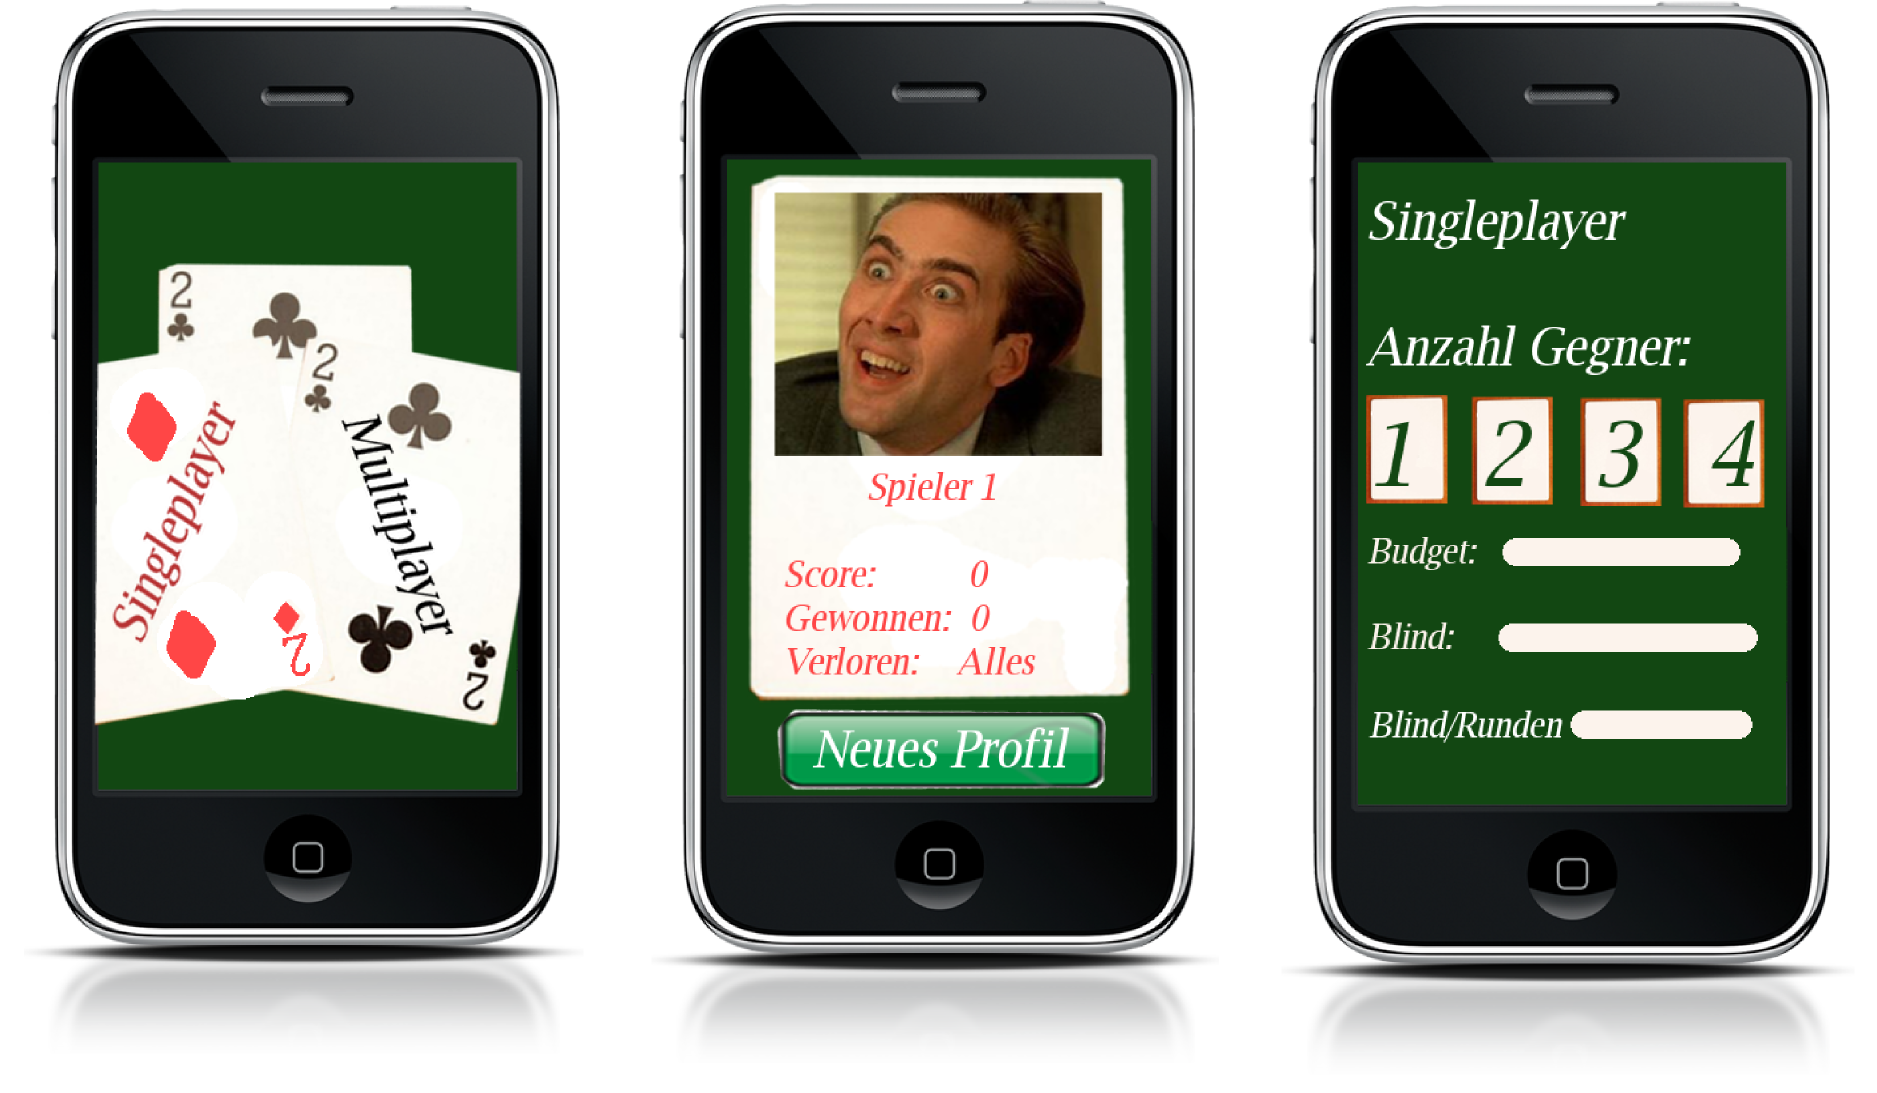
\includegraphics[width=0.8\textwidth]{Fig1}%
\caption{Von links nach rechts: Startbildschirm, Einstellungen, Singleplayermenü}
%\label{Fig1}
\end{figure} 

\begin{figure}[!h]
    \centering
    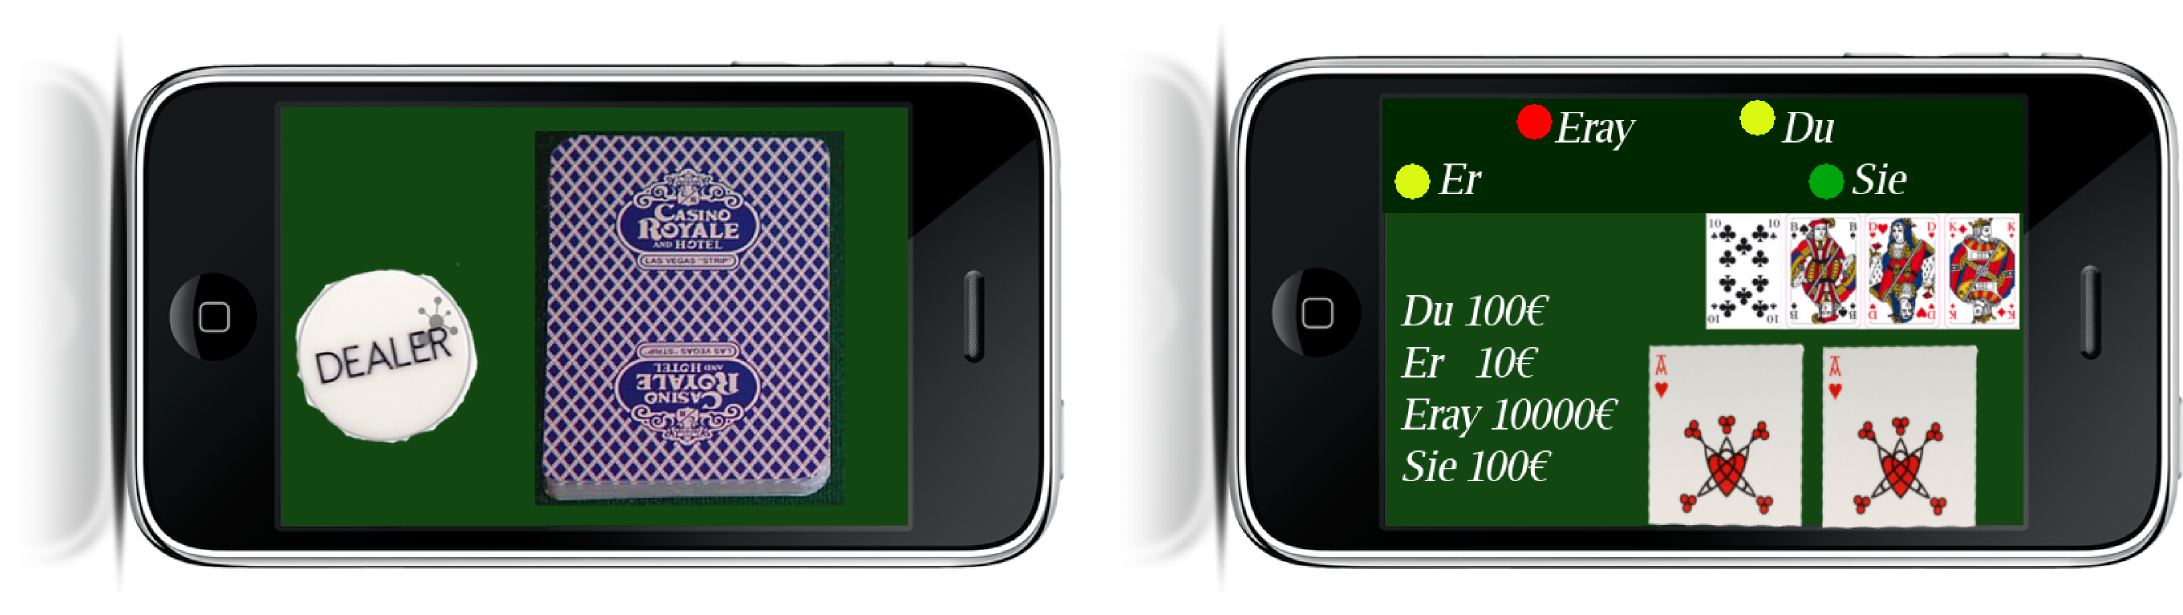
\includegraphics[width=0.8\textwidth]{Fig2}%
\caption{Spielszenen}
%\label{Fig2}
\end{figure} 



\newpage

\section{Entwicklungsumgebung}
Xcode 4

\end{document}






















